\documentclass[11pt]{article}

\usepackage[margin=1in]{geometry}
\usepackage{array}
\usepackage{booktabs}
\usepackage{listings}
\usepackage{tikz}
\usepackage{xcolor}
\usepackage{textcomp}
\usetikzlibrary{positioning,shapes.multipart}

% Colors used in SQL and terminal examples.
\definecolor{codegreen}{rgb}{0,0.55,0}
\definecolor{codepurple}{rgb}{0.50,0,0.70}
\definecolor{backcolour}{rgb}{0.95,0.95,0.92}

\lstdefinestyle{mystyle}{
    backgroundcolor=\color{backcolour},
    commentstyle=\color{codegreen},
    keywordstyle=\color{blue},
    stringstyle=\color{codepurple},
    basicstyle=\ttfamily\footnotesize,
    breakatwhitespace=false,
    breaklines=true,
    captionpos=b,
    keepspaces=true,
    numbers=left,
    numbersep=5pt,
    showspaces=false,
    showstringspaces=false,
    showtabs=false,
    tabsize=2
}

\lstset{style=mystyle}

\title{SQLite Tutorial 3: From a Wide Table to the EAV Model}
\author{Dr. Frank Xu}
\date{\today}

\begin{document}

\maketitle

\section*{Introduction}

A contact can have many attributes: a name, several phone numbers, several email
addresses, and other values. We will begin with the most obvious design: one
table containing one column for each attribute. After using that table, we will
identify its limitations and redesign it so that each attribute is stored as a
separate row. This second approach is called the
\textbf{Entity--Attribute--Value (EAV) model}.

The example uses readable table and column names so that the relationships and
design tradeoffs are easy to follow.

\subsection*{Learning objectives}

After completing this tutorial, you should be able to:

\begin{itemize}
    \item create a contact table that stores all attributes in one row;
    \item compare a wide-table design with an EAV design;
    \item explain the entity, attribute, and value parts of the EAV model;
    \item use identifier columns to connect related tables;
    \item insert multiple attributes for one contact;
    \item join three tables to reconstruct a readable contact; and
    \item search for individual contact attributes.
\end{itemize}

\section*{Step 1: Create and Open the Database}

Open a terminal in the tutorial directory and create a database named
\texttt{contacts.db}:

\begin{lstlisting}[language=bash]
sqlite3 contacts.db
\end{lstlisting}

Make query results easier to read:

\begin{lstlisting}[language=SQL]
.headers on
.mode column
.nullvalue NULL
\end{lstlisting}

\section*{Step 2: Begin with One Contact Table}

The simplest design places every attribute in the same row. We will call this
table \texttt{contacts\_flat} because its columns do not refer to other tables.

\begin{lstlisting}[language=SQL]
CREATE TABLE contacts_flat (
    contact_id   INTEGER PRIMARY KEY,
    account_name TEXT NOT NULL,
    name         TEXT NOT NULL,
    phone        TEXT,
    email        TEXT
);

INSERT INTO contacts_flat
    (contact_id, account_name, name, phone, email)
VALUES
    (101, 'Personal', 'John Smith',
     '+1 555-1234', 'john@gmail.com');
\end{lstlisting}

Querying the contact is straightforward because all of its values are in one
row:

\begin{lstlisting}[language=SQL]
SELECT * FROM contacts_flat;
\end{lstlisting}

\begin{verbatim}
contact_id  account_name  name        phone        email
----------  ------------  ----------  -----------  --------------
101         Personal      John Smith  +1 555-1234  john@gmail.com
\end{verbatim}

This design is easy to create and read when the possible attributes are fixed
and each attribute occurs at most once per contact.

\section*{Step 3: Add a Second Phone Number}

Suppose John has another phone number. The table has only one \texttt{phone}
column, so there is no place to store it as a separate value. One possible fix
is to add another column:

\begin{lstlisting}[language=SQL]
ALTER TABLE contacts_flat ADD COLUMN phone2 TEXT;

UPDATE contacts_flat
SET phone2 = '+1 555-9876'
WHERE contact_id = 101;

SELECT contact_id, name, phone, phone2
FROM contacts_flat;
\end{lstlisting}

\begin{verbatim}
contact_id  name        phone        phone2
----------  ----------  -----------  -----------
101         John Smith  +1 555-1234  +1 555-9876
\end{verbatim}

This solves the immediate problem, but a third number would require
\texttt{phone3}, and a fourth would require \texttt{phone4}. Contacts with only
one number would leave the extra columns \texttt{NULL}. Adding addresses or
other new attributes would require still more schema changes.

Storing several numbers in one text value, such as
\texttt{+1 555-1234, +1 555-9876}, is also undesirable. SQLite would treat the
combined value as one item, making individual numbers harder to search, update,
or count. We therefore need a design that adds rows instead of columns.

\section*{The Entity--Attribute--Value (EAV) Design}

The second approach is an EAV design. The \textbf{entity} is the contact in
\texttt{contacts}. The \textbf{attribute} is the kind of information, such as
\texttt{Name} or \texttt{Phone}, identified in \texttt{attributes}. The
\textbf{value} is the actual name, phone number, or email address stored in
\texttt{data.value}.

The EAV design uses the following tables:

\begin{center}
\begin{tabular}{@{}>{\raggedright\arraybackslash}p{0.18\textwidth}
                    >{\raggedright\arraybackslash}p{0.38\textwidth}
                    >{\raggedright\arraybackslash}p{0.36\textwidth}@{}}
\toprule
Table & Important columns & Purpose \\
\midrule
\texttt{contacts} & \texttt{contact\_id}, \texttt{account\_name}
    & Identifies a contact and its source account \\
\texttt{data} & \texttt{data\_id}, \texttt{contact\_id}, \texttt{attribute\_id}, \texttt{value}
    & Stores one attribute per row \\
\texttt{attributes} & \texttt{attribute\_id}, \texttt{attribute\_name}
    & Defines each available attribute \\
\bottomrule
\end{tabular}
\end{center}

Figure~\ref{fig:contacts-er} shows the two one-to-many relationships. One
contact can own zero or more data rows, and one attribute can describe zero
or more data rows. For these relationships to remain meaningful, every
\texttt{contact\_id} and \texttt{attribute\_id} in \texttt{data} should match a row
in the corresponding table. This tutorial uses matching identifiers but does
not add database constraints to enforce the matches.

\begin{figure}[htbp]
\centering
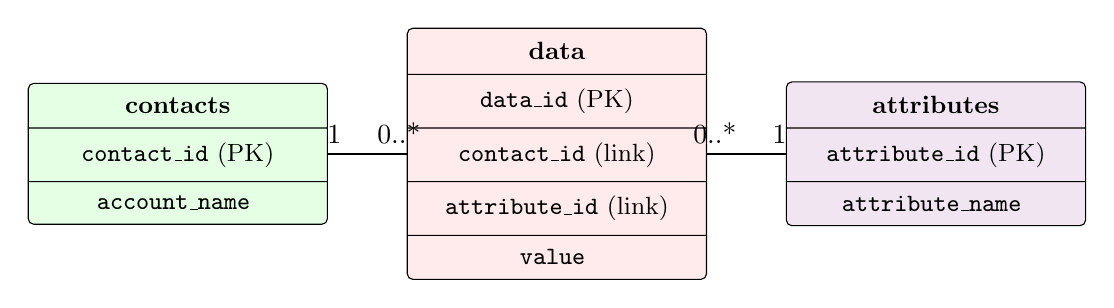
\begin{tikzpicture}[
    entity/.style={
        rectangle split,
        draw,
        rounded corners=2pt,
        align=left,
        font=\small,
        minimum width=3.8cm,
        inner sep=5pt
    },
    relation/.style={draw, thick}
]
\node[entity, rectangle split parts=3, fill=green!10] (contacts) {
    \textbf{contacts}
    \nodepart{second}\texttt{contact\_id} (PK)
    \nodepart{third}\texttt{account\_name}
};

\node[entity, rectangle split parts=5, fill=red!8,
      right=1.0cm of contacts] (data) {
    \textbf{data}
    \nodepart{second}\texttt{data\_id} (PK)
    \nodepart{third}\texttt{contact\_id} (link)
    \nodepart{fourth}\texttt{attribute\_id} (link)
    \nodepart{five}\texttt{value}
};

\node[entity, rectangle split parts=3, fill=violet!10,
      right=1.0cm of data] (attributes) {
    \textbf{attributes}
    \nodepart{second}\texttt{attribute\_id} (PK)
    \nodepart{third}\texttt{attribute\_name}
};

\draw[relation] (contacts.east) --
    node[pos=0.08, above] {1}
    node[pos=0.90, above] {0..*}
    (data.west);
\draw[relation] (data.east) --
    node[pos=0.10, above] {0..*}
    node[pos=0.92, above] {1}
    (attributes.west);
\end{tikzpicture}
\caption{ER diagram for the EAV design. PK denotes a primary
key, and the linking columns connect \texttt{data} to the other tables.}
\label{fig:contacts-er}
\end{figure}

In the EAV design, \texttt{data.value} stores \texttt{John Smith}. The
\texttt{attribute\_id} column links this value to the \texttt{Name} row in
\texttt{attributes}. A second phone number requires one more row rather than a
new column.

\section*{Step 4: Create the EAV Tables}

Create the lookup table first, followed by the parent and child tables:

\begin{lstlisting}[language=SQL]
CREATE TABLE attributes (
    attribute_id   INTEGER PRIMARY KEY,
    attribute_name TEXT NOT NULL UNIQUE
);

CREATE TABLE contacts (
    contact_id   INTEGER PRIMARY KEY,
    account_name TEXT NOT NULL
);

CREATE TABLE data (
    data_id    INTEGER PRIMARY KEY,
    contact_id INTEGER NOT NULL,
    attribute_id INTEGER NOT NULL,
    value      TEXT NOT NULL
);
\end{lstlisting}

The \texttt{contact\_id} and \texttt{attribute\_id} columns link each value to a
contact and an attribute. Later queries will use these matching identifiers
to combine rows from the three tables.

The \texttt{account\_name} value makes the contact's source easy to recognize.
A larger production database might place account details in a separate table,
but that extra relationship is not needed for this lesson.

Inspect the completed definitions:

\begin{lstlisting}[language=SQL]
.schema contacts
.schema data
.schema attributes
\end{lstlisting}

\section*{Step 5: Insert the Attributes}

The \texttt{attributes} table is a lookup table. It stores each attribute name
once and gives it a short integer identifier.

\begin{lstlisting}[language=SQL]
INSERT INTO attributes (attribute_id, attribute_name) VALUES
    (1, 'Name'),
    (2, 'Phone'),
    (3, 'Email');
\end{lstlisting}

Verify the rows:

\begin{lstlisting}[language=SQL]
SELECT * FROM attributes ORDER BY attribute_id;
\end{lstlisting}

\begin{verbatim}
attribute_id  attribute_name
------------  --------------
1             Name
2             Phone
3             Email
\end{verbatim}

\section*{Step 6: Insert a Contact and Its Attributes}

Insert the contact first, followed by its name, phone number, and email address:

\begin{lstlisting}[language=SQL]
INSERT INTO contacts (contact_id, account_name)
VALUES (101, 'Personal');

INSERT INTO data (data_id, contact_id, attribute_id, value) VALUES
    (301, 101, 1, 'John Smith'),
    (302, 101, 2, '+1 555-1234'),
    (303, 101, 3, 'john@gmail.com');
\end{lstlisting}

All three rows have \texttt{contact\_id = 101}, so they belong to the same
contact. Their different \texttt{attribute\_id} values identify the values as
a name, a phone number, and an email address.

View the stored rows directly:

\begin{lstlisting}[language=SQL]
SELECT * FROM contacts;
SELECT * FROM data ORDER BY data_id;
\end{lstlisting}

\begin{verbatim}
contact_id  account_name
----------  ------------
101         Personal

data_id  contact_id  attribute_id  value
-------  ----------  ------------  --------------
301      101         1             John Smith
302      101         2             +1 555-1234
303      101         3             john@gmail.com
\end{verbatim}

The \texttt{value} column alone does not explain what a value means. We must
join \texttt{data} with \texttt{attributes} to interpret it. The column
uses SQLite's \texttt{TEXT} storage class because names, email addresses, and
phone numbers can all contain nonnumeric characters. A phone number should not
be stored as an integer because it may contain a plus sign, spaces, or a leading
zero.

\section*{Step 7: Reconstruct a Readable Contact with JOINs}

Join all three tables by following their key relationships:

\begin{lstlisting}[language=SQL]
SELECT c.contact_id,
       c.account_name,
       a.attribute_name,
       d.value
FROM contacts AS c
JOIN data AS d
  ON d.contact_id = c.contact_id
JOIN attributes AS a
  ON a.attribute_id = d.attribute_id
WHERE c.contact_id = 101
ORDER BY d.data_id;
\end{lstlisting}

\begin{verbatim}
contact_id  account_name  attribute_name  value
----------  ------------  --------------  --------------
101         Personal      Name            John Smith
101         Personal      Phone           +1 555-1234
101         Personal      Email           john@gmail.com
\end{verbatim}

The first \texttt{JOIN} finds all attributes owned by contact 101. The second
\texttt{JOIN} converts each numeric \texttt{attribute\_id} into a readable attribute
name.

\section*{Step 8: Store More Than One Value for an Attribute}

The EAV design does not need columns named \texttt{phone1} and
\texttt{phone2}. Add another row for the \texttt{Phone} attribute:

\begin{lstlisting}[language=SQL]
INSERT INTO data (data_id, contact_id, attribute_id, value)
VALUES (304, 101, 2, '+1 555-9876');
\end{lstlisting}

Retrieve all of John's phone numbers:

\begin{lstlisting}[language=SQL]
SELECT d.data_id, d.value AS phone
FROM data AS d
JOIN attributes AS a
  ON a.attribute_id = d.attribute_id
WHERE d.contact_id = 101
  AND a.attribute_name = 'Phone'
ORDER BY d.data_id;
\end{lstlisting}

\begin{verbatim}
data_id  phone
-------  -----------
302      +1 555-1234
304      +1 555-9876
\end{verbatim}

This is the main benefit of the EAV model: one contact can have any number of
attributes without changing the database schema.

\section*{Step 9: Useful Queries}

Find a contact by part of a stored value:

\begin{lstlisting}[language=SQL]
SELECT c.contact_id,
       c.account_name,
       a.attribute_name,
       d.value
FROM data AS d
JOIN contacts AS c ON c.contact_id = d.contact_id
JOIN attributes AS a ON a.attribute_id = d.attribute_id
WHERE lower(d.value) LIKE '%john%';
\end{lstlisting}

The query finds both values containing \texttt{john}, regardless of letter
case:

\begin{verbatim}
contact_id  account_name  attribute_name  value
----------  ------------  --------------  --------------
101         Personal      Name            John Smith
101         Personal      Email           john@gmail.com
\end{verbatim}

Count the number of attributes stored for each contact:

\begin{lstlisting}[language=SQL]
SELECT c.contact_id,
       c.account_name,
       COUNT(d.data_id) AS attribute_count
FROM contacts AS c
LEFT JOIN data AS d
  ON d.contact_id = c.contact_id
GROUP BY c.contact_id, c.account_name
ORDER BY c.contact_id;
\end{lstlisting}

After adding the second phone number, contact 101 has four attribute rows:

\begin{verbatim}
contact_id  account_name  attribute_count
----------  ------------  ---------------
101         Personal      4
\end{verbatim}

Find contacts that have no data rows:

\begin{lstlisting}[language=SQL]
SELECT c.*
FROM contacts AS c
LEFT JOIN data AS d
  ON d.contact_id = c.contact_id
WHERE d.data_id IS NULL;
\end{lstlisting}

This query returns no rows in the current example because contact 101 has four
matching data rows. If a contact were inserted without any attributes, the
query would return that contact.

\section*{Compare the Two Designs}

The wide table is easier for a small, fixed set of attributes, but the EAV
design is more flexible when contacts can have different numbers or kinds of
attributes.

\begin{center}
\begin{tabular}{@{}>{\raggedright\arraybackslash}p{0.20\textwidth}
                    >{\raggedright\arraybackslash}p{0.34\textwidth}
                    >{\raggedright\arraybackslash}p{0.36\textwidth}@{}}
\toprule
Question & One wide table & EAV design \\
\midrule
Where is a name stored? & In the \texttt{name} column
    & In \texttt{data.value} with attribute \texttt{Name} \\
How is a second phone stored? & Add \texttt{phone2} or combine values
    & Insert another \texttt{data} row \\
How is a new attribute added? & Change the table schema
    & Add an attribute definition and a data row \\
How is a contact read? & One simple \texttt{SELECT}
    & A \texttt{JOIN} reconstructs readable values \\
Main tradeoff & Simple but rigid
    & Flexible but requires related tables and joins \\
Value validation & Each attribute has its own column
    & All values share one \texttt{TEXT} column \\
\bottomrule
\end{tabular}
\end{center}

Neither design is automatically correct for every application. The important
lesson is to recognize the tradeoff. When the number and kind of attributes are
fixed, a wide table may be sufficient. When attributes repeat or change over
time, EAV rows avoid repeatedly altering the schema. However, the application
or later queries must interpret and validate values according to their
attributes.

\section*{Try It Yourself}

Complete the following exercises:

\begin{enumerate}
    \item Add a new attribute named \texttt{Address} with an unused
          identifier.
    \item Add a street address for contact 101 as a new row in
          \texttt{data}.
    \item Write a query that returns only email addresses.
    \item Add contact 102 under the \texttt{Work} account with two phone numbers
          and one email address.
    \item Write a query that counts phone numbers for each contact.
    \item Explain why adding a third phone number does not require an
          \texttt{ALTER TABLE} statement in the EAV design.
\end{enumerate}

\section*{Summary}

The \texttt{contacts} table identifies the owner of a set of attributes and
provides a readable account name.
The \texttt{data} table stores each attribute as a separate row, and the
\texttt{attributes} table describes what each value means. Matching
identifier columns connect the tables, while JOINs reconstruct the rows into
readable contact information. The EAV design adds phone numbers, email
addresses, and other attributes by inserting rows instead of altering the table
schema, at the cost of additional joins and attribute-aware validation.

Exit SQLite when you are finished:

\begin{lstlisting}[language=SQL]
.exit
\end{lstlisting}

\end{document}
